% Assay -- an adversarial framework for payment security
% Mastercard Innovation Challenge 2026
%
% Build:  python scripts/build_figures.py   (figures + numbers.tex)
%         tectonic docs/submission/writeup.tex
%
% This document quotes no result directly. Every figure is \input from numbers.tex,
% which scripts/build_figures.py regenerates from artifacts/*.json, and every plot is
% rendered from the same files. The walkthrough this is drawn from caught itself three
% separate times quoting a number the pipeline had since moved; a document that types
% its own results will do that again, and one that reads them cannot.

\documentclass[11pt,a4paper]{article}

\usepackage[T1]{fontenc}
\usepackage[utf8]{inputenc}
\usepackage{lmodern}
\usepackage{amsmath}   % \text{} inside math mode
\usepackage[margin=2.4cm]{geometry}
\usepackage{graphicx}
\usepackage{float}     % [H] keeps each figure with the claim it supports
\usepackage{booktabs}
\usepackage{xcolor}
\usepackage{titlesec}
\usepackage{enumitem}
\usepackage{caption}
\usepackage{microtype}
\usepackage[hidelinks]{hyperref}

\definecolor{attack}{HTML}{C9372B}
\definecolor{defend}{HTML}{007B9A}
\definecolor{muted}{HTML}{6B6558}
\definecolor{ink}{HTML}{17150F}

\color{ink}
\captionsetup{font=small,labelfont={bf,color=ink},textfont={color=muted}}
\titleformat{\section}{\normalfont\Large\bfseries}{\thesection}{0.6em}{}
\titleformat{\subsection}{\normalfont\large\bfseries}{\thesubsection}{0.6em}{}
\setlist{itemsep=2pt,topsep=4pt}

\newcommand{\claim}[1]{\textcolor{attack}{\textbf{#1}}}

% Generated by scripts/build_figures.py -- do not edit.
% Every macro below is read from artifacts/*.json at build time, so the prose
% cannot quote a number the pipeline has since moved.

\newcommand{\CorpusRows}{1,852,394}
\newcommand{\CorpusFraud}{9,651}
\newcommand{\CorpusBaseRate}{0.521}
\newcommand{\CorpusCards}{999}
\newcommand{\NumFeatures}{20}
\newcommand{\NumFrozen}{7}
\newcommand{\NumCoupled}{4}
\newcommand{\NumFree}{9}
\newcommand{\AsrFirst}{100.0}
\newcommand{\AsrLast}{100.0}
\newcommand{\LzeroFirst}{4.12}
\newcommand{\LzeroLast}{4.03}
\newcommand{\LzeroRise}{-2}
\newcommand{\QueriesFirst}{275}
\newcommand{\QueriesLast}{391}
\newcommand{\QueriesRise}{+42}
\newcommand{\PrAucTemporal}{0.947}
\newcommand{\NTrainTemporal}{907,675}
\newcommand{\SweepRows}{1,852,394}
\newcommand{\NTrainStratified}{907,675}
\newcommand{\PrAucStratified}{0.9457}
\newcommand{\DosageMin}{1}
\newcommand{\DosageMax}{5000}
\newcommand{\DosageWorstPrAuc}{0.7343}
\newcommand{\DosagePrAucDrop}{22.3}
\newcommand{\WidestBudget}{10}
\newcommand{\WidestAsr}{99.8}
\newcommand{\WidestDeclines}{10,035}
\newcommand{\AdvHoldoutBefore}{0.0}
\newcommand{\AdvHoldoutAfter}{68.9}
\newcommand{\AdvTrainAfter}{100}
\newcommand{\AdvRealBefore}{89.3}
\newcommand{\AdvRealAfter}{87.9}
\newcommand{\AdvDeclinesBefore}{114}
\newcommand{\AdvDeclinesAfter}{94}
\newcommand{\AdvHoldoutN}{283}
\newcommand{\ImpossibleShare}{99.9}
\newcommand{\LatencyPFifty}{0.035}
\newcommand{\LatencyPNine}{0.145}
\newcommand{\LatencySamples}{1,000}


\title{\vspace{-1.5cm}\textbf{Assay}\\[0.25cm]
\large Red-teaming payment fraud detection under the constraints
that make a number mean something}
\author{Mastercard Innovation Challenge 2026}
\date{\today}

\begin{document}
\maketitle
\thispagestyle{empty}

\begin{abstract}
\noindent
A fraud detector that scores well offline can be walked past. We built a red team that may
move only what a real attacker controls, against a detector that retrains on every evasion
it finds, and ran the loop until it stopped telling us anything new. Three rounds in, the
attacker still succeeds on \claim{every single attempt} --- so what we report is not a
defeated attack but the price the attacker pays, the price the defender pays, and an audit
showing that an unconstrained attacker's identical-looking score is mostly transactions that
could never occur. We then applied the same loop to a second surface, a payment agent under
indirect prompt injection, and measured it on two model vendors. The most useful results in
this document are the ones that went against us, and Section~\ref{sec:bts} is about those.
\end{abstract}

\begin{center}
\small\itshape
An assay is the test that determines the true metal content of a coin. This framework
does the same to a security number: two attackers report the same 100\% success rate,
and 99.9\% of one's evasions turn out to be base metal.
\end{center}

\begin{center}
\small
\textbf{Live prototype}\quad \url{https://assay-payments.vercel.app}
\par\smallskip
\textbf{Code}\quad \url{https://github.com/Aditya-Patil27/assay}
\end{center}

\noindent
\small\emph{Two pages of the prototype run for real rather than rendering a finished run:
\texttt{/live} downloads the trained detector into the browser and runs the attack against
it, and \texttt{/agent} fires a prompt injection at a live model with the defences on or
off. The repository and deployment keep the \texttt{adversarial-payments} slug they were
created under.}\normalsize

\vspace{0.3cm}

\section{Executive summary}

The framework is a closed loop --- attack, measure, defend, re-measure --- applied to two
attack surfaces that share one contract and one scorecard.

\begin{itemize}
  \item \textbf{The corpus is real.} \CorpusRows{} transactions across \CorpusCards{} cards,
        \CorpusFraud{} of them labelled fraud, a base rate of \CorpusBaseRate\%. That base
        rate is why every detection number here is PR-AUC and recall at a fixed
        false-positive budget, never accuracy.
  \item \textbf{The attack is constrained.} All \NumFeatures{} detector inputs are assigned a
        tier: \NumFrozen{} frozen, \NumCoupled{} coupled as a single merchant move, \NumFree{}
        free. The attacker may touch only the last group, clipped to bands observed in the
        corpus.
  \item \textbf{Attack success does not fall.} It is \AsrFirst\% at round~0 and \AsrLast\% at
        the final round. What moved is the \emph{search} cost: median queries to find an
        evasion \QueriesFirst{} $\to$ \QueriesLast{} (\QueriesRise\%). The number of features
        an evasion touches did not move (\LzeroFirst{} $\to$ \LzeroLast{}, \LzeroRise\%) ---
        retraining made evasions harder to \emph{find}, not structurally more expensive.
  \item \textbf{We refuted our own explanation for that.} Our first draft blamed the flat
        result on too small an adversarial dosage. A sweep from \DosageMin$\times$ to
        \DosageMax$\times$ on the full corpus leaves attack success at \AsrLast\% in every
        arm and every round, while costing \DosagePrAucDrop\% of PR-AUC.
  \item \textbf{The defence does detect the attacks it was trained on the shape of.} On
        \AdvHoldoutN{} adversarial examples the retrained model never saw, recall goes
        \AdvHoldoutBefore\% $\to$ \AdvHoldoutAfter\%, while real-fraud recall holds
        (\AdvRealBefore\% $\to$ \AdvRealAfter\%) and legitimate declines fall from
        \AdvDeclinesBefore{} to \AdvDeclinesAfter{} per 100k. \emph{Measured on a
        \AdvRows-row subsample}, not the full corpus the bullets above use --- the two are
        separate runs and are not a single experiment.
\end{itemize}

\noindent
Those last two bullets are not in tension, and the distinction is the most important one in
this document. \emph{Detecting the attacks we generated} and \emph{withstanding a fresh
search against the retrained model} are different questions. The defence answers the first
and does not answer the second.

\section{The threat landscape}

Pillar~I asks for breadth. We surveyed the vectors below and state plainly which two we
implemented end to end, rather than letting a reader discover the difference.

\begin{itemize}
  \item \textbf{Synthetic identity synthesis} --- fabricated identities aged into
        creditworthiness, defeating per-application checks that never see the cohort.
  \item \textbf{Deepfake-enabled impersonation} --- voice and video cloning against
        call-centre and video-KYC step-up, where the challenge assumes a human is hard to
        imitate live.
  \item \textbf{Localised social engineering at scale} --- UPI collect-request abuse and
        ``digital arrest'' scams, where the authorised-push-payment loss is a genuine
        authorisation the customer was manipulated into making.
  \item \textbf{Agentic prompt injection} --- untrusted text in memos, merchant names and
        dispute evidence, read by an LLM that also holds payment tools.
        \textbf{Implemented (Section~\ref{sec:agentic}).}
  \item \textbf{Adversarial evasion of the detector} --- gradient-free search over the
        features an attacker actually controls. \textbf{Implemented
        (Section~\ref{sec:results}).}
\end{itemize}

\noindent
We deliberately did not build a third surface. Two working surfaces beat three broken ones
under a three-day clock, and the breadth this pillar wants costs writing time rather than
engineering time.

\section{What we built}

\subsection{The contract the attacker is held to}

The central claim of the project is that an adversarial metric means nothing apart from the
constraints it was computed under. So the constraints are data, not prose: every input
column is assigned a tier and a band measured from the corpus (Figure~\ref{fig:constraints}).

\begin{figure}[H]
  \centering
  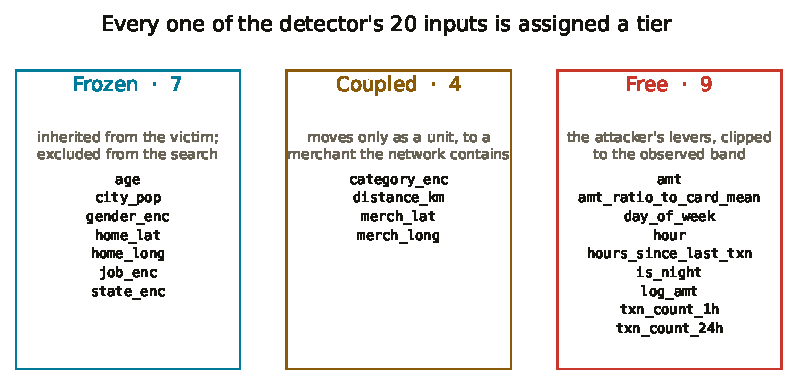
\includegraphics[width=\textwidth]{figures/constraints.pdf}
  \caption{The attack's search space. Frozen columns are inherited from the victim and
  excluded outright; the coupled group can only move to a merchant the network was observed
  to contain; free columns are clipped to their observed band. ``Feasible'' is therefore a
  measured property of the network rather than an assertion by whoever wrote the attack.}
  \label{fig:constraints}
\end{figure}

\subsection{Why this matters for the reported rate}

Running the same search without those projections produces an identical-looking success
rate, of which \ImpossibleShare\% are transactions that could not physically occur --- a
merchant category paired with terminal coordinates no merchant occupies. The headline number
is the same; the thing it describes is not. We run that audit against our own baseline
before reporting anything.

\section{Results}
\label{sec:results}

\subsection{The loop}

\begin{figure}[H]
  \centering
  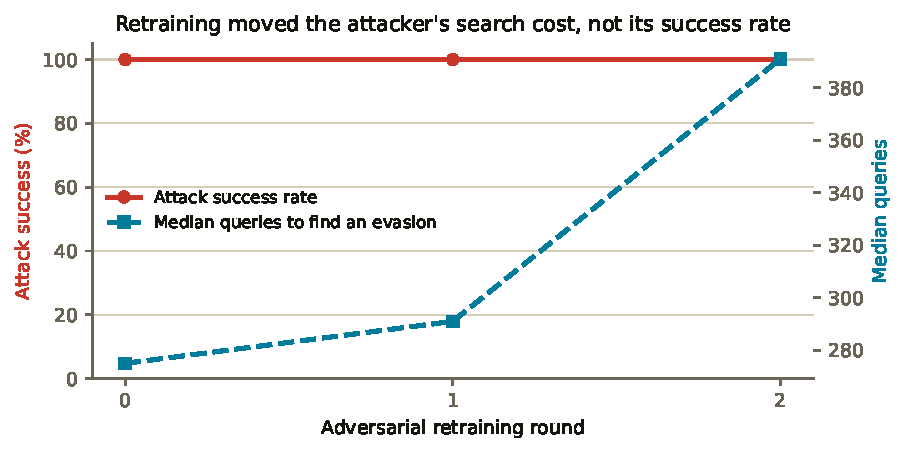
\includegraphics[width=\textwidth]{figures/coevolution.pdf}
  \caption{Attack success is flat at \AsrLast\% across every round, while the search needed
  to reach it lengthens: median queries \QueriesFirst{} $\to$ \QueriesLast{}. Sparsity is
  unchanged over the same rounds (\LzeroFirst{} $\to$ \LzeroLast{}), so the honest reading is
  that retraining made evasions harder to \emph{find} rather than structurally more costly.
  A defence that raises the price of an attack without preventing it is a real outcome, and
  reporting it as a fall in success rate would have been the easier story.}
  \label{fig:coevolution}
\end{figure}

\noindent
The detector behind this loop reports PR-AUC \LoopPrAuc{} at
$n_{\text{train}}=\text{\LoopNTrain}$. Detection quality and attack success are measured on
different axes and are never combined into a single score.

\paragraph{What that number is measured on, because it is not our cleanest split.}
Every aggregate feature in the pipeline is computed causally --- sorted by time, using only
a card's prior transactions --- so none of these results carries label leakage. The
\emph{split} is a separate question and we are not fully clean on it. The unrolled loop
splits stratified at random, which lets a card's other transactions sit on both sides, so
the model can learn card-specific behaviour it would not have at deployment. That is an
easier test set, not leakage, and the rounds above carry it.

We treat a suspiciously high score as a bug report rather than a success. On this data
anything above roughly \(0.95\) PR-AUC suggests leakage, and \LoopPrAuc{} sits just under
that line, on the split most likely to inflate it. \claim{We report it with the caveat
attached rather than quoting the number alone.}

\subsection{We refuted our own excuse}

The obvious objection to Figure~\ref{fig:coevolution} is that we simply did not retrain hard
enough. We tested it rather than argued it.

\begin{figure}[H]
  \centering
  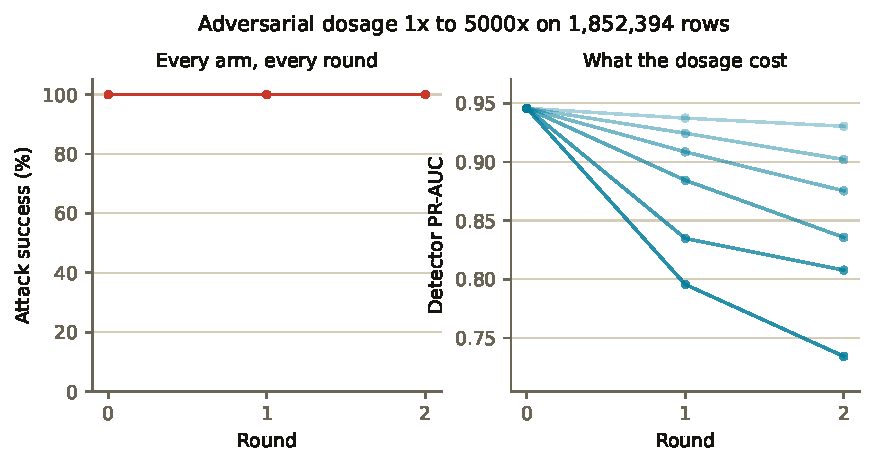
\includegraphics[width=\textwidth]{figures/dosage.pdf}
  \caption{Adversarial dosage swept \DosageMin$\times$ to \DosageMax$\times$ on all
  \SweepRows{} rows ($n_{\text{train}}=\NTrainStratified$). Attack success is
  \AsrLast\% in all 18 measurements. Detector PR-AUC falls from \PrAucStratified{} to
  \DosageWorstPrAuc{}, a \DosagePrAucDrop\% loss. Turning the dial up 5000-fold buys nothing
  and costs a fifth of the detector's quality.}
  \label{fig:dosage}
\end{figure}

\subsection{Nor can the defender simply decline more}

The second obvious objection is that the operating point was too permissive. That is also
testable, and the bill arrives in customer experience.

\begin{figure}[H]
  \centering
  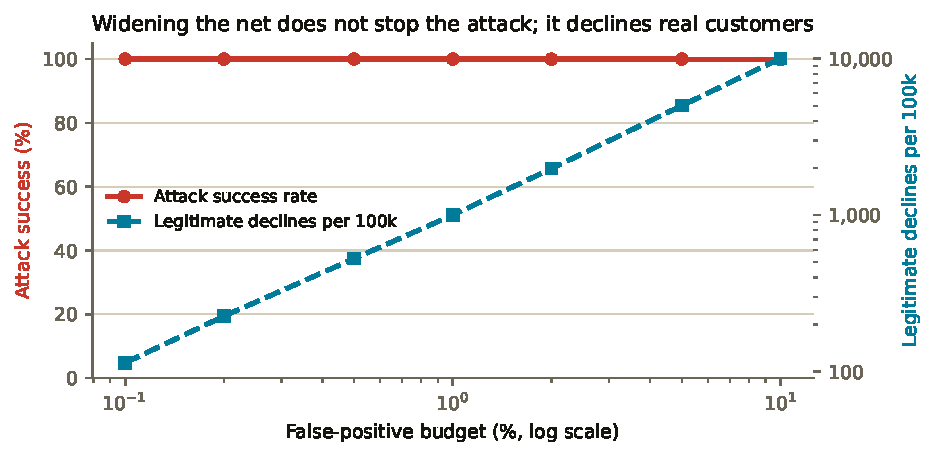
\includegraphics[width=\textwidth]{figures/threshold.pdf}
  \caption{Attack success against the false-positive budget. It holds at \AsrLast\% until
  the budget reaches \WidestBudget\%, where it falls only to \WidestAsr\% --- at a cost of
  \WidestDeclines{} legitimate declines per 100{,}000 transactions. There is no threshold at
  which this attack stops being viable and the business still has customers.}
  \label{fig:threshold}
\end{figure}

\subsection{What the defence does achieve}

Adversarial retraining is not worthless, and the distinction is precise.

\begin{figure}[H]
  \centering
  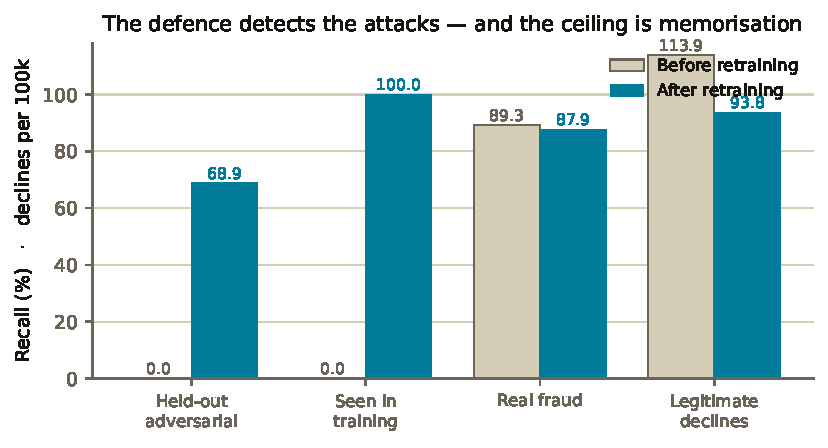
\includegraphics[width=\textwidth]{figures/adversarial_detection.pdf}
  \caption{Recall on \AdvHoldoutN{} adversarial examples the retrained model never saw:
  \AdvHoldoutBefore\% $\to$ \AdvHoldoutAfter\%. Recall on adversarial rows it \emph{did} see
  is \AdvTrainAfter\%, which is the memorisation ceiling and is why the held-out figure is
  the only honest one. Real-fraud recall holds and legitimate declines fall. Measured on a
  \AdvRows-row subsample; the co-evolution and sweep figures use the full corpus.}
  \label{fig:advdet}
\end{figure}

\noindent
So: the retrained detector catches attacks of a shape it has seen, generalising to unseen
instances of that shape, without costing real-fraud recall or customer experience. It does
not stop a fresh search. Both statements are true and only the pair is honest.

\section{The second surface: agentic prompt injection}
\label{sec:agentic}

A payment agent reads untrusted text --- memos, merchant display names, dispute evidence ---
and holds tools that move money. We planted injections in exactly those channels and scored
them by OWASP LLM Top~10 category, with three defence layers: an injection classifier, tool
scoping, and a human-in-the-loop threshold.

\begin{figure}[H]
  \centering
  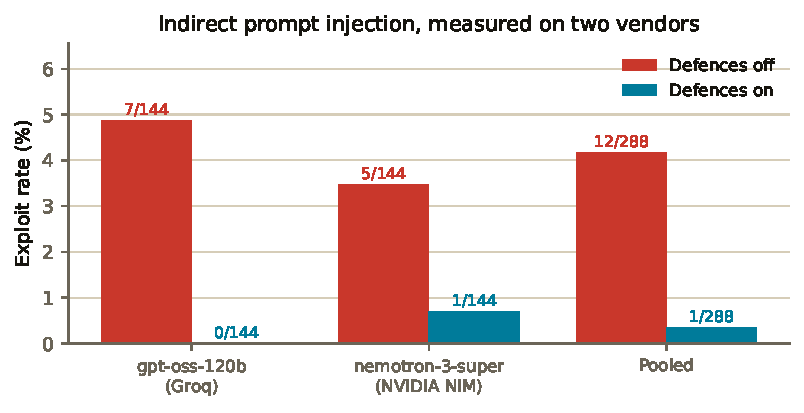
\includegraphics[width=\textwidth]{figures/agentic.pdf}
  \caption{Exploit rate before and after the defence layer, on two vendors. Two-sided Fisher
  exact on each row's own $2\times2$ table: gpt-oss-120b $p=0.015$, nemotron-3-super
  $p=0.214$, pooled $p=0.003$. The reduction clears $\alpha=0.05$ on one model and on the
  pooled corpus, and does not clear it on the other. We report all three.}
  \label{fig:agentic}
\end{figure}

\noindent
An earlier run at half this corpus size reported the same reduction as not significant. That
was correct at $n=72$ and is superseded at $n=144$ per arm. \emph{The defence did not change;
the statistical power did}, and we say so rather than quietly replacing one number with a
better one.

\section{Real-world feasibility}

The detector is exported to ONNX and measured on the serving path: \LatencyPFifty~ms at p50
and \LatencyPNine~ms at p99 over \LatencySamples{} single-transaction calls. That is inside
an authorisation budget by three orders of magnitude.

The web prototype runs the same trained ensemble in the browser by walking its 400 trees
directly, which is a \emph{different execution path} from the server-side ONNX figure above
and is not what that latency describes. The two are held equal by a conformance check rather
than by assumption (Section~\ref{sec:repro}).

\section{Behind the scenes: four measurement errors we caught in our own work}
\label{sec:bts}

Every number in this document looked entirely reasonable at the moment it was wrong. None of
the errors below was caught by a figure looking implausible; each was caught by asking what
the number had been measured \emph{under}. That is the thesis of the project, applied to
ourselves.

\subsection{An attack that succeeded by surrendering the money}

An early engine reported \AsrLast\% success --- achieved by shrinking transactions to roughly
12\% of their value. An attacker who gives up 88\% of the take to avoid detection has not
defeated the system; they have been priced out of it. Adding an economic floor moved
retained attacker value from 11.4\% to 74.5\%, and changed the attack's shape: the flawed
version reached for the amount lever in 57 of 60 successes, the corrected one spreads across
amount, timing and merchant choice.

\subsection{A missing measurement rendered as a confident zero}

The dashboard plotted detector quality per round and substituted \texttt{0} where a round had
not been trained. It drew detection quality collapsing to the axis, directly beneath a caption
saying detection quality holds --- with the correct value displayed two inches away. The cause
was one defaulting expression, \texttt{?? 0}, which converts \emph{``I have no measurement''}
into \emph{``I measured zero''}.

\claim{A missing measurement presented as a confident zero is not a smaller error than a
fabricated result. It is a fabricated result, produced automatically.} The fix was not a
better default but the removal of the default: the value is nullable, absent rounds are drawn
absent, and the table names them ``not run''.

\subsection{A threshold fitted on the test split}

The loop chose its operating threshold by maximising F1 on the test split --- contradicting
our own documented policy, and fitting the operating point on the rows the attack was then
scored against. It lifted the bar to roughly 0.94 against a budget-derived cut near 0.23, and
raised it further every round, so each round of ``defence'' quietly handed the attacker an
easier target than the last.

The honest part is the outcome: fixing it made evasion genuinely harder, and attack success
stayed at \AsrLast\% anyway. The bug was not propping up the result. Had we found it after
publishing, the number would have survived --- but we would have been quoting it for the
wrong reason and could not have told the difference.

\subsection{We refuted our own excuse}

The draft explained the flat attack success rate as an artefact of small adversarial dosage.
Figure~\ref{fig:dosage} is the test of that explanation, and it fails: 5000$\times$ the
dosage changes nothing and costs \DosagePrAucDrop\% of PR-AUC. We deleted the excuse rather
than keeping it as a hedge.

\subsection{A fifth, caught while writing this document}

The artifacts moved underneath this writeup mid-draft. An earlier run had mean features
touched rising \(3.81 \to 4.64\); the current one has \LzeroFirst{} \(\to\) \LzeroLast{}.
The prose, the figure and the prototype all said attacker effort was climbing, and one of
the two axes had stopped agreeing.

It was caught mechanically rather than by reading: this document defines every quoted value
as a macro, and a cross-check of defined-versus-referenced macros flagged one that had gone
unused. The template also hard-coded a \texttt{+} before the delta, so a fall would have
rendered as ``+-2\%'' --- a sign error announcing a substantive one. The deltas now carry
their own sign, and the figure plots the axis that actually moved.

\claim{The claim that survives is narrower than the one we had written.} Retraining makes
evasions harder to \emph{find} --- median queries \QueriesFirst{} \(\to\) \QueriesLast{} --- and
does not make them structurally more expensive.

\subsection{Two smaller retractions, same species}

\begin{itemize}
  \item We reported the static export as working from \texttt{file://}. It resolved every
        asset and rendered blank charts, because a cross-origin chunk fails a CORS check
        against an opaque origin. \emph{Assets resolving} and \emph{a page working} are
        different claims and we had checked the first.
  \item The live agent demo opened on an injection/scenario pair where nothing happened in
        either condition --- only 7 of 144 pairs exploit gpt-oss-120b undefended. A judge
        would have concluded the demo was broken rather than that the model held. It now
        opens on a pair that actually exploits.
\end{itemize}

\section{Reproducibility}
\label{sec:repro}

The same logic exists in two languages three separate times, and each pair is held equal by
a check that fails loudly rather than by good intentions.

\begin{center}
\begin{tabular}{@{}lll@{}}
\toprule
\textbf{Guarantee} & \textbf{Covers} & \textbf{Command} \\
\midrule
Artifact contract cannot drift & 10 mirrored interfaces & \texttt{pytest tests/test\_artifacts.py} \\
Live agent runs the corpus defences & 144 documents, 360 spans & \texttt{npm run check:agent} \\
Browser detector is the trained model & 68 rows, agreement to $10^{-6}$ & \texttt{npm run check:trees} \\
Fixture data announces itself & 14 enveloped artifacts & \texttt{pytest} \\
\bottomrule
\end{tabular}
\end{center}

\noindent
Every artifact carries a placeholder flag, a git SHA and a timestamp. While any figure on
the prototype is seeded fixture data, a banner names the exact files --- so no number on the
site can quietly be invented. Every figure in this document is generated by
\texttt{scripts/build\_figures.py} from those same artifacts.

\section{Limitations}

\begin{itemize}
  \item Attack success does not fall. We report the cost imposed instead, and we tested and
        rejected the two obvious explanations for why it does not fall.
  \item The adversarial-detection result generalises to unseen instances of a shape the model
        has seen. It is not evidence against a fresh adaptive search.
  \item The agentic result is significant on one vendor and on the pooled corpus, and not on
        the other vendor. All three are reported.
  \item The corpus is a public simulation of card transactions, not production data from a
        live rail.
\end{itemize}

\end{document}
